\documentclass{article}
\usepackage{tikz}
\usepackage[utf8]{inputenc}
\usepackage[T1]{fontenc}
% Pour des icônes plus détaillées si désiré (pas strictement nécessaire pour cet exemple)
\usepackage{etoolbox}

% Définition de couleurs personnalisées
\definecolor{myorange}{RGB}{242, 133, 46}
\definecolor{myblack}{RGB}{0, 0, 0}

% Configuration de TikZ
\usetikzlibrary{shapes,positioning,calc,arrows.meta}

\tikzset{
    % Styles globaux
    >={Stealth[length=3mm, width=1.5mm]}, % Style de flèche par défaut
    microgrid_bus/.style={line width=2pt, black},
    power_flow_arrow/.style={-latex, myorange, line width=0.8pt},
    device_base/.style={inner sep=1pt, outer sep=0pt},
    label_base/.style={font=\small\sffamily},
    label_orange/.style={label_base, color=myorange},
    label_black/.style={label_base, color=black},
    comp_icon/.style={draw, thin, fill=gray!10, rounded corners=2pt, minimum width=1cm, minimum height=1cm, inner sep=0pt},
}

\begin{document}

\centering
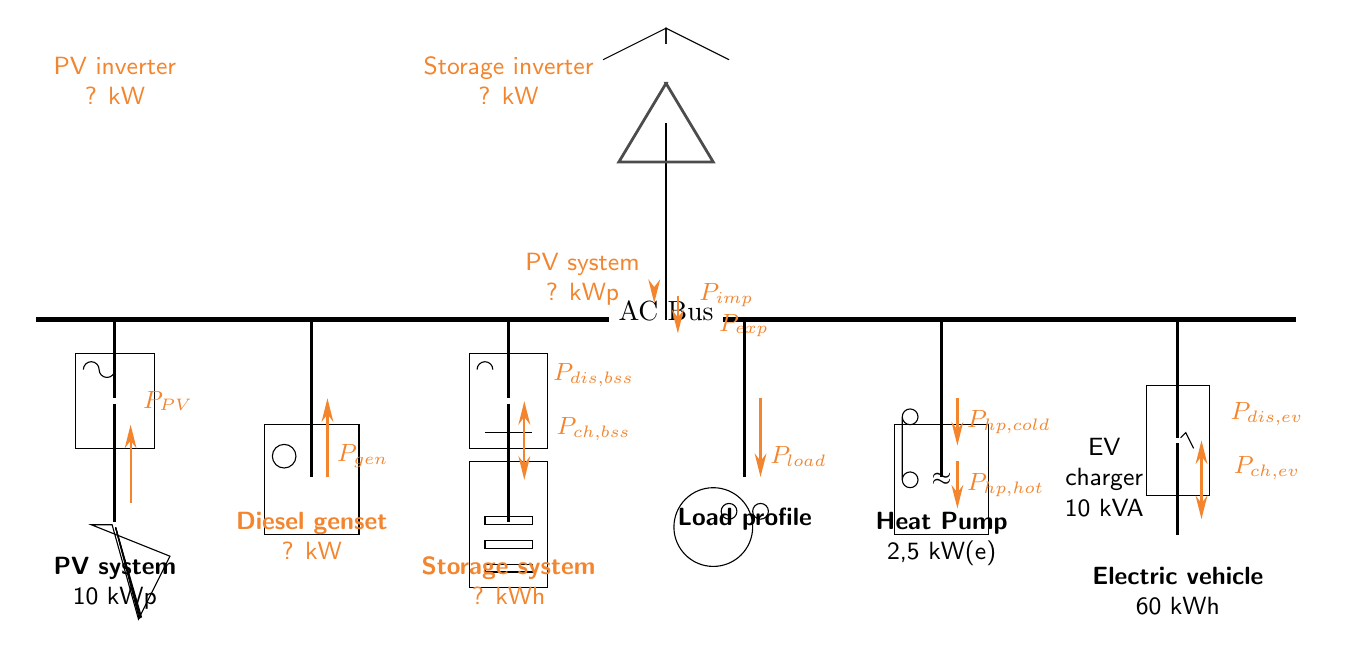
\begin{tikzpicture}[node distance=0.5cm and 0.5cm, scale=1.0, transform shape]

% === Structure principale (Le Bus AC) ===
\coordinate (ACbus_left) at (-8, 0);
\coordinate (ACbus_right) at (8, 0);
\draw[microgrid_bus] (ACbus_left) -- (ACbus_right) node[midway, above=3pt, anchor=center, fill=white] {AC Bus};

% === Positions clés sur le bus (pour les connexions) ===
% Nous créons des points d'attache sur le bus
\foreach \i/\name in {-7/PV, -4.5/GEN, -2/BAT, 1/LOAD, 3.5/HP, 6.5/EV} {
    \coordinate (bus_\name) at (\i, 0);
}

% === 1. Connection au Réseau (Pylône) ===
% Pylône simplifié
\coordinate (pylon_pos) at (0, 3);
\draw[line width=1pt] (0,0) -- (0, 2.5); % Connexion verticale
\draw[line width=1pt, draw=black!70] (0,2.5) ++(0,0.5) -- ++(-0.6, -1) -- ++(1.2, 0) -- ++(-0.6, 1) -- cycle; % Tête
\draw[thin] (0,2.5) ++(0,1) -- ++(0,0.2) -- ++(-0.8, -0.4); % Câbles
\draw[thin] (0,2.5) ++(0,1) -- ++(0,0.2) -- ++(0.8, -0.4);

% Texte et flèches de flux (Pimp/Pexp)
\node[label_orange, above left] (label_imp) {
    \begin{tabular}{c}
        PV system\\
        ? kWp
    \end{tabular}
};
\draw[power_flow_arrow, <-] ([xshift=-1.5mm, yshift=-3mm]label_imp.east) -- ([xshift=-1.5mm, yshift=3mm]label_imp.east |- bus_LOAD);
\node[label_orange, right=3mm of label_imp, yshift=-0.2cm] {$P_{imp}$};

\node[label_orange, above right] (label_exp) {};
\draw[power_flow_arrow, ->] ([xshift=1.5mm, yshift=3mm]label_exp.west |- bus_LOAD) -- ([xshift=1.5mm, yshift=-3mm]label_exp.west);
\node[label_orange, right=3mm of label_exp, yshift=-0.2cm] {$P_{exp}$};


% === 2. Branche PV (Panneaux + Onduleur) ===
\node[label_orange] at (bus_PV |- pylon_pos) {
    \begin{tabular}{c}
        PV inverter\\
        ? kW
    \end{tabular}
};
% Onduleur
\node[device_base, below=1cm of bus_PV] (PV_inverter) {};
% Icône simple pour onduleur
\draw[thin] ([xshift=-0.5cm, yshift=-0.6cm]PV_inverter) rectangle ++(1, 1.2);
\draw[thin] ([xshift=-0.4cm]PV_inverter) ++(0, 0.4) arc(180:0:0.1cm) arc(180:360:0.1cm); % Symbole sinusoïdal
% Panneaux
\node[device_base, below=1.5cm of PV_inverter] (PV_panels) {};
\draw[thin] ([xshift=-0.7cm, yshift=-0.8cm]PV_panels) -- ++(0.4, 0.8) -- ++(1.0, -0.4) -- ++(-0.4, -0.8) -- cycle;
\foreach \i in {1,...,4} { \draw[thin] ([xshift={-0.7cm+(\i*1.4/5)}, yshift={-0.8cm+(\i*0.8/5)}]PV_panels) -- ++(1.0,-0.4); }
% Connexions
\draw[line width=1pt] (bus_PV) -- (PV_inverter);
\draw[line width=1pt] (PV_inverter) -- (PV_panels);
% Texte
\node[label_black, below=2mm of PV_panels] {\begin{tabular}{c}\textbf{PV system}\\ 10 kWp\end{tabular}};
% Flux
\draw[power_flow_arrow, <-] ([xshift=2mm, yshift=-3mm]bus_PV |- PV_inverter) -- ++(0, -1cm);
\node[label_orange, right=2mm of PV_inverter] {$P_{PV}$};


% === 3. Branche Diesel (Genset) ===
\node[device_base, below=2cm of bus_GEN] (Diesel_genset) {};
% Icône simple pour Genset (Groupe + Réservoir)
\draw[thin] ([xshift=-0.6cm, yshift=-0.7cm]Diesel_genset) rectangle ++(1.2, 1.4);
\draw[thin] ([xshift=-0.5cm, yshift=0.3cm]Diesel_genset) arc(180:-180:0.15cm); % Échappement
% Connexion
\draw[line width=1pt] (bus_GEN) -- (Diesel_genset);
% Texte
\node[label_orange, below=2mm of Diesel_genset] {\begin{tabular}{c}\textbf{Diesel genset}\\ ? kW\end{tabular}};
% Flux
\draw[power_flow_arrow, <-] ([xshift=2mm, yshift=-1cm]bus_GEN) -- ++(0, -1cm);
\node[label_orange, right=2mm of bus_GEN |- Diesel_genset, yshift=0.3cm] {$P_{gen}$};


% === 4. Branche Stockage (Batterie + Onduleur) ===
\node[label_orange] at (bus_BAT |- pylon_pos) {
    \begin{tabular}{c}
        Storage inverter\\
        ? kW
    \end{tabular}
};
% Onduleur Batterie
\node[device_base, below=1cm of bus_BAT] (BAT_inverter) {};
\draw[thin] ([xshift=-0.5cm, yshift=-0.6cm]BAT_inverter) rectangle ++(1, 1.2);
\draw[thin] ([xshift=-0.4cm]BAT_inverter) ++(0, 0.4) arc(180:0:0.1cm); % AC side
\draw[thin] ([xshift=-0.4cm]BAT_inverter) ++(0.1, -0.4) -- ++(0.6, 0); % DC side
% Batterie
\node[device_base, below=1.5cm of BAT_inverter] (BAT_system) {};
\draw[thin] ([xshift=-0.5cm, yshift=-0.8cm]BAT_system) rectangle ++(1, 1.6);
\draw[thin] ([xshift=-0.3cm, yshift=-0.6cm]BAT_system) rectangle ++(0.6, 0.1); % Barres horizontales
\draw[thin] ([xshift=-0.3cm, yshift=-0.3cm]BAT_system) rectangle ++(0.6, 0.1);
\draw[thin] ([xshift=-0.3cm, yshift=0.0cm]BAT_system) rectangle ++(0.6, 0.1);
% Connexions
\draw[line width=1pt] (bus_BAT) -- (BAT_inverter);
\draw[line width=1pt] (BAT_inverter) -- (BAT_system);
% Texte
\node[label_orange, below=2mm of BAT_system] {\begin{tabular}{c}\textbf{Storage system}\\ ? kWh\end{tabular}};
% Flux
\draw[power_flow_arrow, <->] ([xshift=2mm]bus_BAT |- BAT_inverter) -- ++(0, -1cm);
\node[label_orange, right=2mm of BAT_inverter] {
    \begin{tabular}{c}
        $P_{dis,bss}$\\[3mm]
        $P_{ch,bss}$
    \end{tabular}
};


% === 5. Branche Charge (Prise) ===
\node[device_base, below=2cm of bus_LOAD] (Load_plug) {};
% Icône simple pour prise
\draw[thin] ([xshift=-0.4cm, yshift=-0.6cm]Load_plug) circle (0.5cm);
\draw[thin] ([xshift=-0.2cm, yshift=-0.4cm]Load_plug) circle (0.1cm); % Pins
\draw[thin] ([xshift=0.2cm, yshift=-0.4cm]Load_plug) circle (0.1cm);
% Connexion
\draw[line width=1pt] (bus_LOAD) -- (Load_plug);
% Texte
\node[label_black, below=2mm of Load_plug] {\textbf{Load profile}};
% Flux
\draw[power_flow_arrow, ->] ([xshift=2mm, yshift=-1cm]bus_LOAD) -- ++(0, -1cm);
\node[label_orange, right=2mm of bus_LOAD |- Load_plug, yshift=0.3cm] {$P_{load}$};


% === 6. Branche Pompe à Chaleur (Unité Extérieure) ===
\node[device_base, below=2cm of bus_HP] (Heat_pump) {};
% Icône simple pour PAC
\draw[thin] ([xshift=-0.6cm, yshift=-0.7cm]Heat_pump) rectangle ++(1.2, 1.4);
\draw[thin] ([xshift=-0.5cm, yshift=0cm]Heat_pump) arc(180:-180:0.1cm) -- ++(0,0.8) arc(-180:180:0.1cm) --cycle; % Échangeur
\node at (Heat_pump) {\small \(\approx\)};
% Connexion
\draw[line width=1pt] (bus_HP) -- (Heat_pump);
% Texte
\node[label_black, below=2mm of Heat_pump] {\begin{tabular}{c}\textbf{Heat Pump}\\ 2,5 kW(e)\end{tabular}};
% Flux
\draw[power_flow_arrow, ->] ([xshift=2mm, yshift=-1cm]bus_HP) -- ++(0, -0.6cm);
\draw[power_flow_arrow, ->] ([xshift=2mm, yshift=-1.8cm]bus_HP) -- ++(0, -0.6cm);
\node[label_orange, right=2mm of bus_HP, yshift=-1.3cm] {$P_{hp,cold}$};
\node[label_orange, right=2mm of bus_HP, yshift=-2.1cm] {$P_{hp,hot}$};


% === 7. Branche Véhicule Électrique (Chargeur) ===
% Texte Chargeur
\node[label_black, left=1mm of bus_EV |- Heat_pump] (EV_charger_label) {
    \begin{tabular}{c}
        EV\\
        charger\\
        10 kVA
    \end{tabular}
};
% Icône simple pour borne VE
\node[device_base, below=1.5cm of bus_EV] (EV_charger) {};
\draw[thin] ([xshift=-0.4cm, yshift=-0.7cm]EV_charger) rectangle ++(0.8, 1.4);
\draw[thin] ([xshift=-0.1cm, yshift=-0.3cm]EV_charger) -- ++(0.2, 0.4) -- ++(0.1, -0.2); % Logo foudre
% Ligne verticale pointant vers le bas
\draw[line width=1pt] (EV_charger) -- ++(0, -1.2cm);
% Connexion bus
\draw[line width=1pt] (bus_EV) -- (EV_charger);
% Texte
\node[label_black, below=2mm of EV_charger, yshift=-1.2cm] {\begin{tabular}{c}\textbf{Electric vehicle}\\ 60 kWh\end{tabular}};
% Flux
\draw[power_flow_arrow, <->] ([xshift=3mm]bus_EV |- EV_charger) -- ++(0, -1cm);
\node[label_orange, right=3mm of EV_charger] {
    \begin{tabular}{c}
        $P_{dis,ev}$\\[3mm]
        $P_{ch,ev}$
    \end{tabular}
};

\end{tikzpicture}

\end{document}